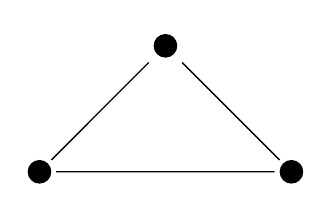
\begin{tikzpicture}[node distance=2cm,scale = .8]
% Vértices
\tikzset{black vertex/.style={circle,draw,minimum size=1mm,inner sep=0pt,outer sep=2pt,fill=black, color=black}}

  \node (0) at (0,0) {0};
  \node[black vertex] () at (0,0) {0};
  \node[black vertex] (1) at (2,-2) {1};
  \node[black vertex] (2) at (-2,-2) {2};

% \draw[line width = .5pt] (0) -- (1) (2) -- (3) (4) -- (5) (6) -- (7) (8) -- (9) (10) -- (11) (12) -- (13) (14) -- (15);

\draw[line width = .5pt] (0) -- (1) (0) -- (2) (1) -- (2) ;

\end{tikzpicture}